\subsection{Planos de Bit}

Extração de um plano de bit $M$ da imagem. O argumento $M$ deve aparecer logo após o comando, como em:

\begin{minted}{bash}
    $ python main.py imagens/baboon.png plano.bit 4
\end{minted}

\begin{listing}[H]
    \caption{Comando \texttt{plano.bit M}}

    \begin{minted}{python}
        def plano_de_bit(imagem, bit):
            plano = (imagem >> bit) & 1
            return plano * 255
    \end{minted}
\end{listing}

\begin{figure}[H]
    \centering
    \begin{subfigure}{0.45\textwidth}
        \centering
        
\includegraphics[width=6cm]{resultados/colorbit.png}
        \caption{\texttt{imagens/color.png}}
    \end{subfigure}%
    \begin{subfigure}{0.45\textwidth}
        \centering
        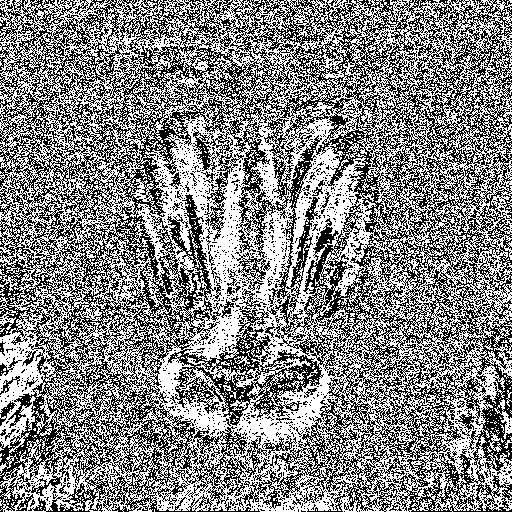
\includegraphics[width=6cm]{resultados/baboonbit.png}
        \caption{\texttt{imagens/babooon.png}}
    \end{subfigure}

    \caption{Plano de bit 4.}
\end{figure}
